\documentclass[10pt]{beamer}
\usepackage{fontspec}
\usepackage{caption}
\usetheme{metropolis}
\definecolor{uiucblue}{HTML}{13294B}
\definecolor{steelblue}{HTML}{4682b4}
\definecolor{skyblue}{HTML}{00bfff}
\definecolor{bananayellow}{HTML}{ffe135}
\definecolor{bluishgreen}{cmyk}{97,0,75,0}
\definecolor{darkpurple}{HTML}{9F4C93}
\definecolor{offwhite}{HTML}{F5F5F5}
\definecolor{bestcolor}{cmyk}{97,0,75,0}
\setbeamercolor{background canvas}{bg=white}
\setbeamercolor{frametitle}{bg=offwhite, fg=black}
\setbeamercolor{block body}{bg=offwhite}
\setbeamercolor{block title}{bg=mDarkTeal!10}
\usepackage{pifont}% http://ctan.org/pkg/pifont
\setlength{\columnsep}{3em}
\def\columnseprulecolor{\color{black}}
\usepackage{amsthm,amsmath,amssymb,bbm,bm}
\usepackage{mathtools}
\usepackage{booktabs}
\usepackage{graphicx}
\usepackage{subcaption}
\usepackage{multicol}
\usepackage{transparent}
\usepackage{xcolor}
\usepackage{colortbl}
\usepackage{tikz}
\usepackage{appendixnumberbeamer}
\newcommand<>{\uncovergraphics}[2][{}]{
    % Taken from: <https://tex.stackexchange.com/a/354033/95423>
    \begin{tikzpicture}
        \node[anchor=south west,inner sep=0] (B) at (4,0)
            {\includegraphics[#1]{#2}};
        \alt#3{}{%
            \fill [draw=none, fill=white, fill opacity=1.0] (B.north west) -- (B.north east) -- (B.south east) -- (B.south west) -- (B.north west) -- cycle;
        }
    \end{tikzpicture}
}

\DeclarePairedDelimiter\set{\{}{\}}
\DeclarePairedDelimiter\floor{\lfloor}{\rfloor}
\DeclarePairedDelimiterX{\norm}[1]{\lVert}{\rVert}{#1}
\DeclareMathOperator*{\bigoh}{\mathcal{O}}
\DeclareMathOperator*{\spn}{span}
\DeclarePairedDelimiterX{\abs}[1]{\lvert}{\rvert}{#1}

\def\mOne{{\mathbbm{1}}}
\newcommand{\ind}[1]{\mOne\{#1\}}

\newcommand{\X}{\mathbf{X}}
\newcommand{\mbx}{\mathbf{x}}
\newcommand{\mbz}{\mathbf{z}}
\newcommand{\Reals}[1]{\mathbb{R}^{#1}}
\newcommand{\condit}{\, | \,}

\newcommand{\Syx}{\mathcal{S}_{Y \condit \X}}

\newcommand{\semitransp}[2][35]{\color{fg!#1}#2}

\newcommand{\LeftChild}{C_{L}}
\newcommand{\RightChild}{C_{R}}

\DeclareMathOperator*{\argmin}{arg\,min}
\DeclareMathOperator*{\argmax}{arg\,max}


% probability
\DeclarePairedDelimiterX{\expectarg}[1]{[}{]}{%
    \,
    \ifnum\currentgrouptype=16 \else\begingroup\fi
    \activatebar#1
    \ifnum\currentgrouptype=16 \else\endgroup\fi
    \,
}
\DeclarePairedDelimiterX{\variancearg}[1]{(}{)}{%
    \,
    \ifnum\currentgrouptype=16 \else\begingroup\fi
    \activatebar#1
    \ifnum\currentgrouptype=16 \else\endgroup\fi
    \,
}
\newcommand{\E}{\mathbb{E} \, \expectarg}
\newcommand{\Ehat}{\widehat{\mathbb{E}} \, \expectarg}
\newcommand{\En}{E_n \, \expectarg}
\newcommand{\cond}{\, | \,}

\newcommand{\EP}{\mathbb{E}_P \, \expectarg}
\newcommand{\Var}{\operatorname{Var}\variancearg}
\newcommand{\Varhat}{\operatorname{\hat{Var}}\variancearg}
\newcommand{\Cov}{\operatorname{Cov}\variancearg}
\newcommand{\CovP}{\operatorname{Cov_P}\variancearg}
\newcommand{\Corr}{\operatorname{Corr}\variancearg}
\newcommand{\innermid}{\nonscript\;\delimsize\vert\nonscript\;}
\newcommand{\activatebar}{%
    \begingroup\lccode`\~=`\|
    \lowercase{\endgroup\let~}\innermid
    \mathcode`|=\string"8000
}
\DeclareMathOperator*{\logit}{logit}
\newcommand{\iid}{\text{iid}}

\newcommand*{\figuretitle}[1]{%
    {
     \textbf{#1}
    \par\medskip}
}

\newcommand{\iidsim}{\overset{\text{iid}}\sim}

\newcommand{\cmark}{\textcolor{orange}{\ding{51}}}
\newcommand{\xmark}{\textcolor{gray}{\ding{55}}}%

\title{The Truncated SPRT}

\author{Anamitra Chaudhuri and Joshua Loyal}
\institute{STAT 578: Sequential Design \\ \\
           Paper: \\
           \textit{Asymptotic Efficiences of Truncated Sequential Tests} \\
           by Sawasd Tantaratana and Harold Vincent Poor}
\date{\today}

\begin{document}

\begin{frame}[noframenumbering, plain]
\titlepage
\end{frame}

\begin{frame}
\frametitle{Problem Setup}

Consider $X_1, X_2, \dots \iidsim f_{\theta}$ where $f_{\theta}(x)$  belongs to the exponential family, i.e  $f_{\theta}(x) = f_0(x) e^{\theta x - \psi(\theta)}$.

Given $\theta_1 > \theta_0$, we want to design a sequential test $(T, D)$ for
\[
H_0: \theta \leq \theta_0 \quad \text{vs.} \quad H_1: \theta \geq \theta_1
\]
such that the error probabilities are controlled at levels $\alpha, \beta$:
\[
P_{\theta_0}(D = 1) \leq \alpha \quad \text{ and } \quad P_{\theta_1}(D = 0) \leq \beta.
\]
\end{frame}

\begin{frame}
\frametitle{Problem Setup}

Often times we employ a sequenial test to collect less samples than the equivalent fixed sample size (FSS) test:

\[
D_{FSS} = \ind{Z_M(\theta_1, \theta_0) \geq \tau}
\]

where $M$ and $\tau$ are chosen to achieve the specified error probabilities ($\alpha, \beta$).

\end{frame}

\begin{frame}
\frametitle{Problem Setup}

The SPRT has a smaller $E_{\theta}(T\,)$ than the FSS for $\theta \notin (\theta_0, \theta_1)$. For $\theta \in (\theta_0, \theta_1)$, the SPRT's ESS can be much larger than the fixed sample size test, e.g.

\begin{figure}
\centering
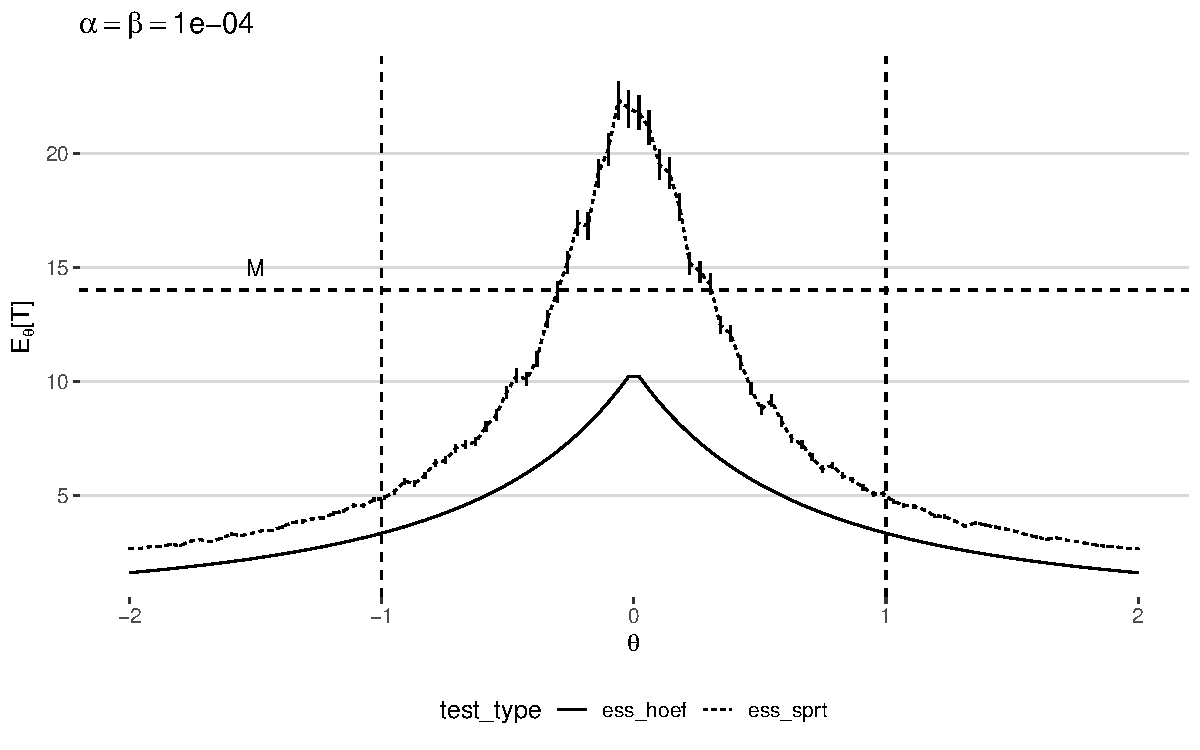
\includegraphics[width=0.7\textwidth]{images/sprt_ess.pdf}
\end{figure}

This is the case for small error probabilities common in many applications!
\end{frame}

\begin{frame}
\frametitle{Problem Setup}

\begin{block}{Goal}
Design a constant boundary truncated sequential test that combines the SPRT with a final FSS test.
\end{block}

\textit{Remark:} We have seen tests with truncated boundaries before, e.g. Lorden's 2-SPRT, GLR, Mixture, etc.
\begin{itemize}
\item Achieve truncation through non-constant (intersecting) boundaries.
\item The derivation of the (non-constant) boundaries can be difficult to derive in general.
\item The truncation point is often very large.
\end{itemize}

%As long as we know how to acheive the desired error control, a test that combines and SPRT with a constant FSS boundary is easy to implement.

\end{frame}

\begin{frame}
\frametitle{The Truncated SPRT}

\begin{figure}
\centering
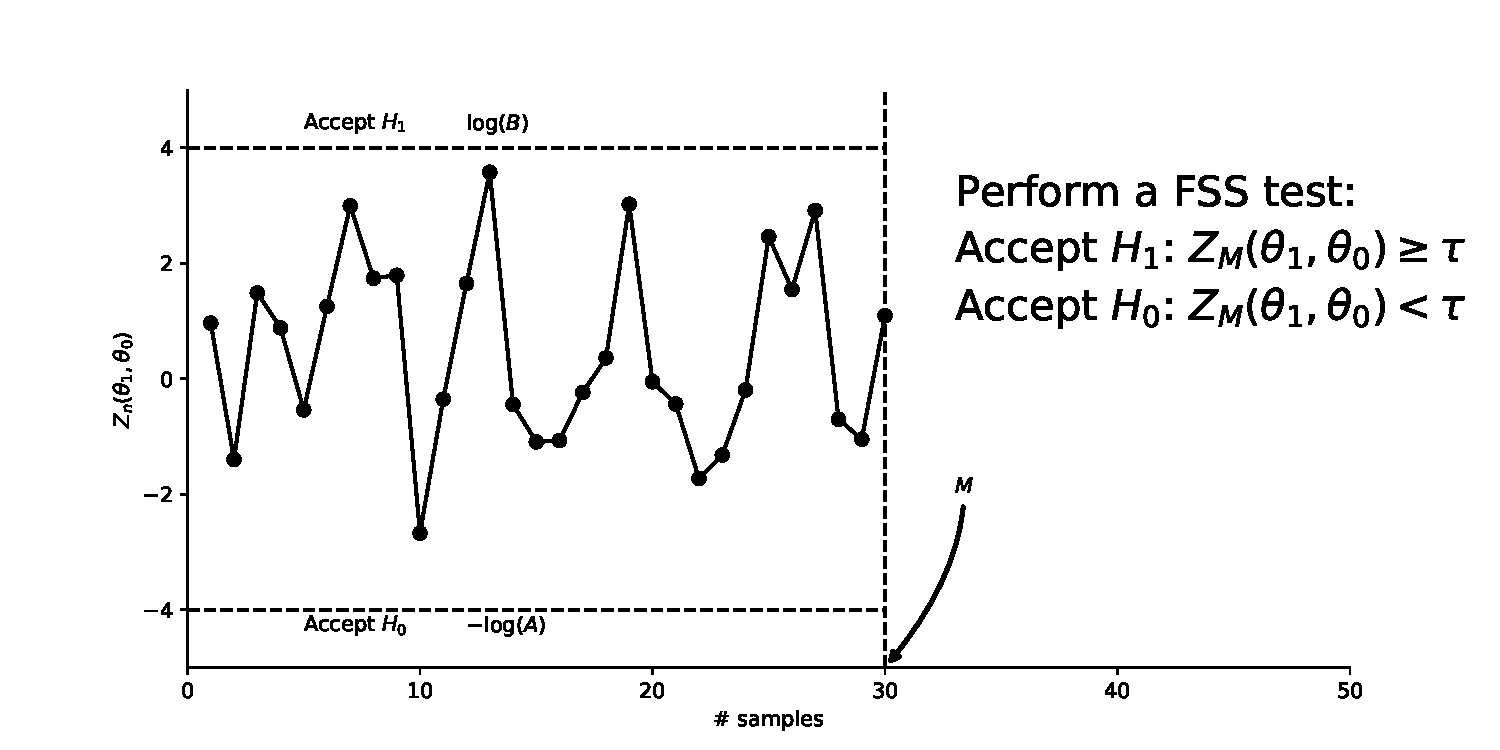
\includegraphics[width=\textwidth]{images/truncated_sprt}
\end{figure}

\end{frame}

\begin{frame}
\frametitle{The Truncated SPRT}

Formally, let $T_{SPRT} = \inf\set{n \geq 1 : Z_{T}(\theta_1, \theta_0) \notin (-\log(A), \log(B)) }$.

Set $T = T_{SPRT} \wedge M$. The decision rule is
\[
D =
\begin{cases}
1  & T < M \text{ and } Z_T \geq log(B) \text{ or } T = M \text{ and } Z_M \geq \tau \\
0  & T < M \text{ and } Z_T \leq -log(A) \text{ or } T = M \text{ and } Z_M < \tau .
\end{cases}
\]

\begin{figure}
\centering
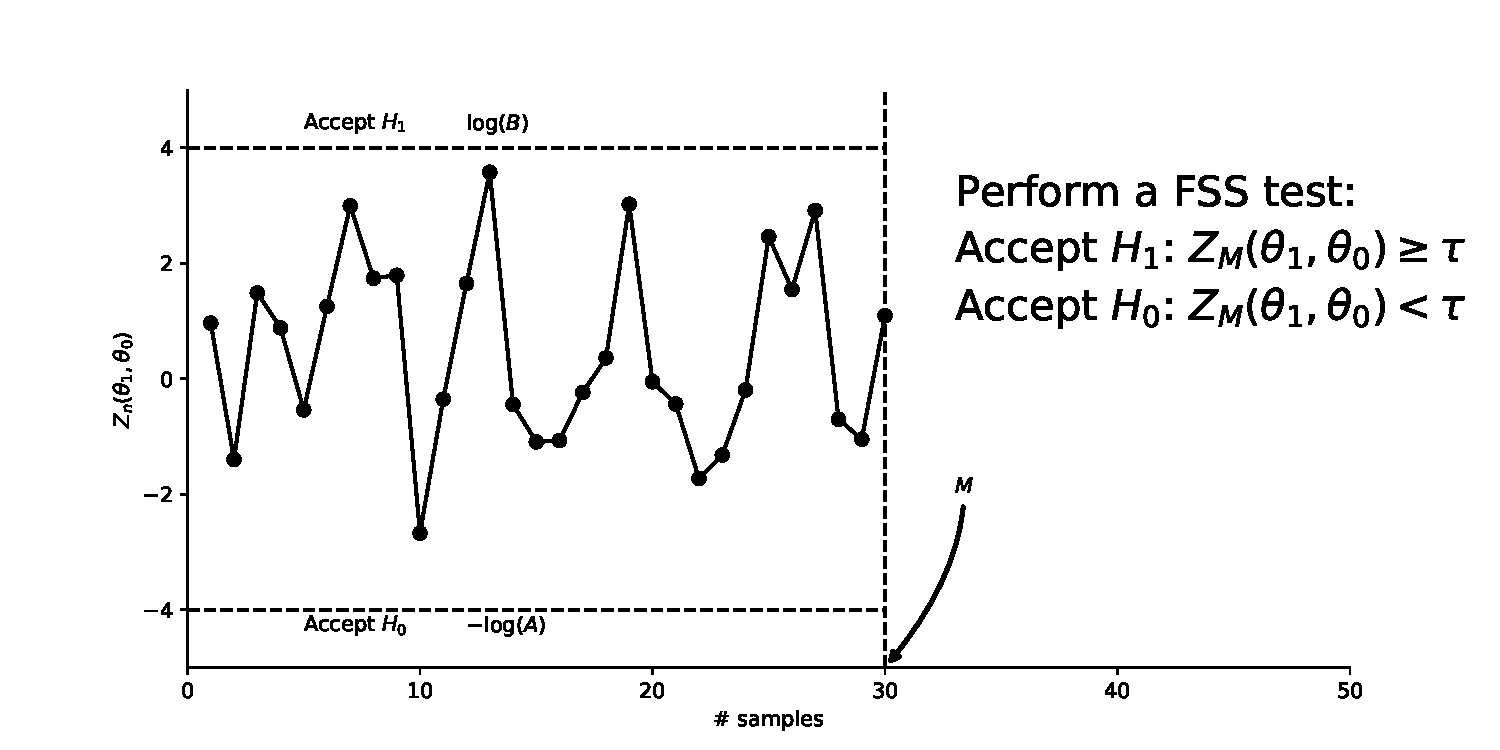
\includegraphics[height=0.5\textheight, width=0.8\textwidth]{images/truncated_sprt}
\end{figure}
\end{frame}


\begin{frame}
\frametitle{The Truncated SPRT}
\textbf{Outstanding Questions}

\begin{itemize}
\item How do we choose $A, B, M, \tau$ to acheive the desired error control?
\item Does the ESS of the truncated SPRT fall below the equivalent $M_{FSS}$ once we acheive the desired error control?
\item How does this test compare with other truncated tests: Lorden's 2-SPRT and the GLR?
\end{itemize}

\end{frame}

\begin{frame}
\frametitle{Design of the Truncated SPRT}

\begin{block}{Lemma}
\[
\begin{split}
P_{\theta_0}(D = 1) &\leq \alpha_{SPRT} + \alpha_{FSS} \\
P_{\theta_1}(D = 0) &\leq \beta_{SPRT} + \beta_{FSS}
\end{split}
\]
\end{block}

\textit{Proof:}
\[
\begin{split}
P_{\theta_0}(D = 1) &= P_{\theta_0}(T < M, Z_T \geq \log(B)) + P_{\theta_0}(T = M, Z_M \geq \tau) \\
    &\leq P_{\theta_0}(Z_T \geq \log(B)) + P_{\theta_0}(Z_M \geq \tau) \\
    &= \alpha_{SPRT} + \alpha_{FSS}
\end{split}
\]

Similarly, $\beta \leq \beta_{SPRT} + \beta_{FSS}$.

\end{frame}

\end{document}
